\documentclass[
 prl,
 twocolumn,
 amsmath,
 amssymb,
 aps,
]{revtex4-2}

\usepackage{colortbl}
\usepackage{graphicx} 
\usepackage{booktabs}
\usepackage{caption}
\usepackage{notes2bib}
\newcommand{\red}{\textcolor{red}}
\usepackage[justification=raggedright]{caption}

\captionsetup{justification=Justified}

\begin{document}

\title{Beyond May: Complexity-stability relationships \\
in disordered dynamical systems}

\author{Onofrio Mazzarisi}
\affiliation{Department of Ecology and Evolutionary Biology, University of Kansas,
Higuchi Hall, 2101 Constant Avenue, Lawrence, KS 66047, USA}

\author{Matteo Smerlak}
\affiliation{Laboratoire Biophysique et Evolution, ESPCI ParisTech, 10 rue Vauquelin, 75005 Paris, France}
\affiliation{Capital Fund Management, 23 Rue de l'Université, 75007 Paris, France}


\date{\today}

\begin{abstract}
Robert May famously used random matrix theory to predict that large, complex systems cannot admit stable fixed points. 
Unfortunately, this general conclusion is not supported by empirical observation: from cells to biomes, biological systems are large, complex---and, by and large, stable.
In this paper, we revisit May's argument in the light of recent developments in both ecology and random matrix theory. 
Using a non-linear generalization of the Lotka-Volterra model, we show that there are in fact two kinds of complexity-stability relationships in disordered dynamical systems: 
if self-interactions grow faster with density than cross-interactions, complexity is destabilizing; but if cross-interactions grow faster than self-interactions, complexity is stabilizing.
Our result shows that May's principle that "complexity begets instability" is not a general property of complex systems; instead, it is a property of a subclass of weakly cross-regulated disordered systems.
\end{abstract}
\maketitle

%Introduction
\paragraph*{}

Few mathematical arguments have influenced biological thinking like May's prediction that large, complex ecosystems cannot be stable~\cite{May1972}.
It is a perplexing conclusion.
On the one hand, May's mathematical argument is simple and seemingly model-free, suggesting universal applicability, also outside biology \cite{Haldane2011, Moran2019}.
On the other hand, it is clear that at least some large, complex systems are stable---else which regularities would biology by studying in the first place? Empirically, the opposite relationship between complexity and stability seems to hold across ecosystems: species-rich, strongly-coupled communities such as rainforests tend to be stable over time, while sparser ones, for instance arctic communities, often exhibit large fluctuations, exctinctions, and invasions~\cite{Hutchinson1959,Odum1959,MacArthur1955}. 
The tension between May's theoretical argument and  observation is at the center of the longlasting "diversity-stability debate" in ecology \cite{McCann2000, Loreau2022}.

May's argument can be summarized as follows.
A system with $N$ populations $x_i$ is stable is one that can be characterized by an equilibrium point $\mathbf x^*$.
Near that equilibrium $\mathbf x = \mathbf x^* + \delta \mathbf x$, the dynamics of the system is described by linear equations $d(\delta \mathbf x)/dt = A (\delta \mathbf x)$, and the stability of these equations requires that all eigenvalues of $A$ have negative real part.
But if $A$ can be represented as $A = B - I$, where $B$ consists of random, independent interactions (with zero 
mean and variance $\sigma^2$), and $-I$ corresponds to stabilizing self-interactions on some natural timescale, 
then the circular law of random matrix theory implies that all eigenvalues of $A$ will have negative real part only if $\sigma^2 N < 1$.
This places a sharp constraint on both diversity $N$ and interaction strengh $\sigma$, often referred to as "complexity begets instability".
(This argument generalizes to $\langle B_{ij}\rangle \neq 0$, incomplete connectivity, to correlated interactions, see e.g. \cite{allesina2015stability}.)

In ecology, many authors have sought to ease the tension between May's 
prediction and empirical observation by invoking effects not captured by 
dynamical systems with random 
coefficients~\cite{McCann2000,Chesson2000,Mougi2012,Rohr2014,Barabas2017,Grilli2017}. In this letter, we use recent results in the physics of disordered systems \cite{Ahmadian2015, Roy2019} to show that May's argument itself is incomplete: 
random dynamical systems do not necessarily imply that 
stability decreases with dimensionality and interaction 
strength---the opposite behavior is also possible, 
without the need for special or additional structure.

%Model
\paragraph*{}
\emph{Model.---}Consider the dynamical system in $N$ variables
\begin{equation}\label{dynamics}
    \dot{x}_i = f(x_i) + \sum_{j}A_{ij}g(x_i)h(x_j) \, .
\end{equation}
Here $f(x_i)$ represents the self-interaction of a population $i$, while $g(x_i)$ and $h(x_j)$ capture the cross-interaction of $i$ with other populations. That interaction is weighted by a coefficient $A_{ij}$, such that $A_{ij} > 0$ (resp.
$A_{ji} < 0$) implies a positive (resp.
negative) effect of $j$ on the growth of $i$. 
We assume all of $f$, $g$ and $h$ are increasing functions, and refer to $f$ as the ``production function'' and $g$ as the ``response function''.

This rather general setting has been used to study universality in network dynamics \cite{Barzel2013} and to construct minimal models for complex dynamics \cite{Barzel2015}, with applications ranging from biological~\cite{Alon2006,Karlebach2008} 
to social~\cite{Pastor-Satorras2001,Hufnagel2004,Dodds2005} systems.

The classic generalized Lotka-Volterra (GLV) competition model studied recently by Bunin and collaborators \cite{bunin2017ecological, biroli2018marginally} corresponds to $f$, $g$, $h$ all linear. 
However, it is natural both physically and biologically to consider more general functions, including power laws $f(x)\sim x^\alpha$, $g(x)\sim x^\beta$, $h(x) \sim x^\gamma$.
From a physical perspective, we can imagine populations $x_i$ forming three-dimensional clusters whose growth is limited to their two-dimensional surface, leading to a production function $f(x) \sim x^{2/3}$.
Biologically, the growth of organisms (populations of cells) has long been known to scale like $f(x) \sim x^k$ with $k\simeq 3/4$~\cite{Brown2004}, which can be understood in terms of hydrodynamic constraints on vascular and pulmonary networks.
For reasons that are not currently understood, a similar pattern of growth appears to recur at the community level~\cite{Hatton2015,Hatton2023}.
In a different direction, it has been recently suggested that predator-prey interactions can be modelled with a square root law ($g(x) \sim h(x) \sim x^{1/2}$)~\cite{Barbier2021,Mazzarisi2023}.


%Homogeneous interactions
\paragraph*{}
\emph{Homogeneous interactions.---}Under what condition does~\eqref{dynamics} admit a (linearly) stable equilibrium? 
We begin with the simple case where all self-interactions have the same strength $A_{ii} = \mu_s$, and similarly for cross-interactions $A_{ij} = \mu$ ($i\neq j$).
Defining 
\begin{equation}
    \psi(x) \equiv (\mu_s - \mu) -  \left(\frac{f'(x)}{f(x)} - \frac{g'(x)}{g(x)}\right)\frac{f(x)}{g(x)h'(x)},
    \label{eq: psi}
\end{equation}
an elementary calculation shows that stability of the homogeneous equilibrium $x_i^* = x^*$ requires $\psi(x^*)g(x^*)h'(x^*) > 0$, or $\psi(x^*)>0$ if we assume that $g$ and $h$ are positive, increasing functions. This stability condition involves the relative strength of diagonal and off-diagonal interactions ($\mu_s - \mu$), but also on the relative growth rate of the production and response functions near the equilibrium ($f'(x^*)/f(x^*) - g'(x^*)/g(x^*)$).

With power laws, the condition $\psi(x^*)>0$ evaluates to 
\begin{equation}
    (\alpha - \beta)(N-1) < \gamma(\mu_s/\mu- 1) - (\alpha - \beta)(\mu_s/\mu),
\end{equation}
leading to three different regimes:
\begin{itemize}
    \item If $\alpha = \beta$, stability requires $\mu_s > \mu$, i.e.
    self-interactions must be stronger than cross-interactions.
    This is the usual conclusion drawn from the Lotka-Volterra model.
    \item If $\alpha > \beta$, stability places an upper bound on $N$: the more complex the system, the less likely to be stable.
    We can call this ``May" behavior.
    \item If $\alpha < \beta$, stability places an lower bound on $N$: the more complex the system, the more likely to be stable.
    This is ``anti-May" behavior.
\end{itemize}


%Random interactions: stability condition
\paragraph*{}
\emph{Random interactions: stability condition.---}We now consider the case of random interactions.
Specifically, we assume that interaction coefficients $A_{ij}$ are drawn independently from a distribution with mean $\mu$ and standard deviation $\sigma$;
We assume the diagonal elements $A_{ii}$ have a mean value $\mu_s$ (possibly different from $\mu$) but the same standard deviation $\sigma$. 
 
We compute the Jacobian matrix at equilibrium
\begin{align}
    J_{ij}^* & = - A_{ij}g(x_i^*)h'(x_j^*) \qquad \qquad \textrm{for} \ i\neq j \label{eq: jac off-diag}\\
    J_{ii}^* & = f'(x_i^*) - g'(x_i^*)f(x_i^*)/g(x_i^*) - A_{ii}g(x_i^*)h'(x_j^*) \ , \label{eq: jac diag}
\end{align}
where we used $\sum_{j}A_{ij}h(x_j^*)=f(x_i^*)/g(x_i^*)$.
In order to investigate the spectral properties of $J^*$, 
we follow Stone~\cite{Stone2018} in using a recent generalization of the circular law in random matrix theory~\cite{Ahmadian2015}.

In Ref.~\cite{Ahmadian2015}, Ahmadian \emph{et al.} consider matrices of the form $M + LSR$, where $M$,  
$L$ and $R$ are deterministic matrices, and $S$ is a random matrix with i.i.d. coefficients, zero mean and variance $\sigma^2$.
They show that eigenvalues of large matrices of this form are contained in the complex domain $\mathcal{D} = \{\zeta \in \mathbb{C},\, \textrm{Tr}[(\Psi(\zeta) \Psi(\zeta)^\dagger)^{-1}]\geq \sigma^{-2}\}$, where $\Psi(\zeta) = L^{-1}(M-\zeta I)R^{-1}$. If $L$, $R$ and $M$ are all diagonal $N\times N$ matrices, the equation of $\mathcal{D}$ simplifies to 
\begin{equation}
    \sum_{i=1}^N\Big\vert\frac{M_{ii} - \zeta}{L_{ii}R_{ii}}\Big\vert^{-2}\geq \sigma^{-2}.
\label{eq: domain}
\end{equation}

To use this result, we decompose the interaction matrix as $A = \mu\mathbf{1} + (\mu_s-\mu)I + S$,
with $\mathbf{1}$ the matrix with all entries equal to $1$ and $S$ a random matrix as defined above.
Up to the rank-one perturbation $\mu\mathbf{1}$ which does not affect stability properties \cite{Stone2018}, we can write the Jacobian~\eqref{eq: jac off-diag} as $J = M + LSR$ with diagonal matrices
\begin{equation}
    M_i = - g(x_i^*)h'(x_i^*)\psi(x_i^*),\quad L = g(x_i^*), \quad R = h'(x_i^*),
\end{equation}
where $\psi(x)$ is the function defined in~\eqref{eq: psi}. 
\begin{figure}[t!]
    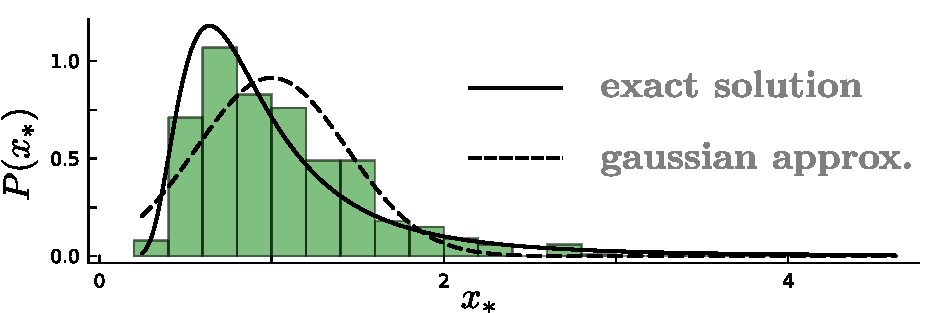
\includegraphics[width=.45\textwidth]{figs/cavity.pdf}
    \caption{The equilibrium distribution with power-law self- and cross-interactions is accurately reproduced by 
    Eq.~\eqref{eq: dist general} and its Gaussian approximation.
    For simulations (in green) we used $\alpha=1$, $\beta=3/2$,
    $\gamma=1$, $N=50$, $\mu=\mu_s=10^{-2}$, $\sigma=5\cdot 10^{-3}$.}
    \label{fig: cavity sol.}
\end{figure}
Stability of the equilibrium requires that $\mathcal{D}$ be entirely contained in the left half-plane (all eigenvalues have negative real part). For this to hold, it is no longer sufficient that $\psi(x_i^*) > 0$ for each $i$: we must also have that $0\notin \mathcal{D}$, hence from~\eqref{eq: domain}:
\begin{equation}
    \sum_{i=1}^N \Big(\frac{\sigma}{\psi(x_i^*)}\Big)^{2}
    < 1.
    \label{eq: random-stability}
\end{equation}
In the GLV model, $\psi(x) = \mu_s - \mu$ (independently of $x$) and we recover the classical condition $\sigma\sqrt{N} < (\mu_s-\mu)$ \footnote{In fact, the same condition holds when $f$ and $g$ are power laws with the same exponent.}. In general, however, the dependence on equilibrium values $x_i^*$ (which in turn depend on $N$) does not cancel out, and one must gain information about the distribution of equilibrium values $P(x_i^*)$ to assess the stability condition~\eqref{eq: random-stability}.

%Random interactions: equilibrium distribution
\paragraph*{}
\emph{Random interactions: equilibrium distribution.---}Henceforth we assume $f(x_i)=x_i^{\alpha}$, $g(x_i)=x_i^{\beta}$, $h(x_i)=x_i^{\gamma}$. 
(Any coefficients can be reabsorbed in the statistics of $A$ and by a rescaling of time.)
\begin{figure}[t!]
    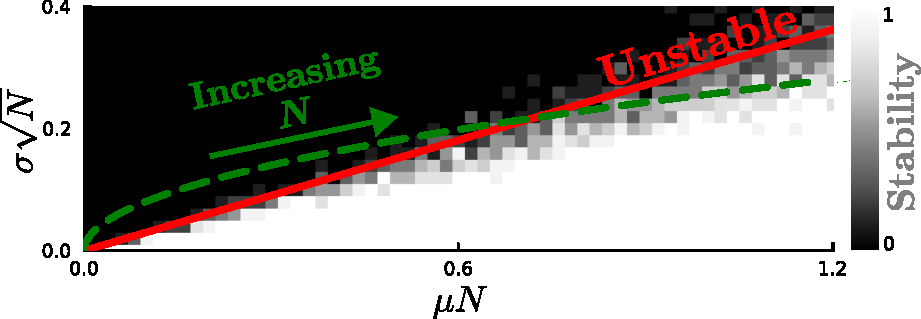
\includegraphics[width=.45\textwidth]{figs/beta1_5-S50-N10-diversity-increase.pdf}
    \caption{For a system in the ``anti-May" phase, an increase in $N$,
    corresponding to moving along $\sqrt{N}$ in the $(\sigma \sqrt{N},\mu N)$ plane (green dashed line), will be stabilizing rather than destabilizing.
    Here we show results from the numerical resolution of the dynamical system~\eqref{dynamics}. Stability is defined as full stable coexistence. The red line is computed obtained using DMFT and the generalized stability condition $N\langle (\sigma/\psi)^2\rangle < 1$.
    Parameters values are $\alpha=1$, $\beta=3/2$,
    $\gamma=1$, $N=50$ and $10$ replicates for the simulations. For the line representing the increase in $N$ we fixed $\mu=0.1$ and $\sigma=0.75$.}
    \label{fig: stability line + sims}
\end{figure}
Following e.g. Ref.~\cite{Roy2019}, we can derive from the evolution equation~\eqref{dynamics} a dynamical mean field theory (DMFT) 
which describes the ensemble of $N\gg 1$ variables
by means of a single, self-consistent representative stochastic trajectory
\begin{equation}
    \dot{x} = x^{\alpha}-A_sx^{\beta+\gamma}-x^{\beta}\big( \mu N \langle x^{\gamma}\rangle + \sigma \sqrt{N} \eta\big) \, ,
\label{eq: dmft}
\end{equation}
where $A_s$ is a random variable with the statistics of $A_{ii}$ and $\eta$ is a Gaussian noise with zero mean and correlation $\langle x^{\gamma}(t)x^{\gamma}(s)\rangle$. 
\begin{figure}[t!]
    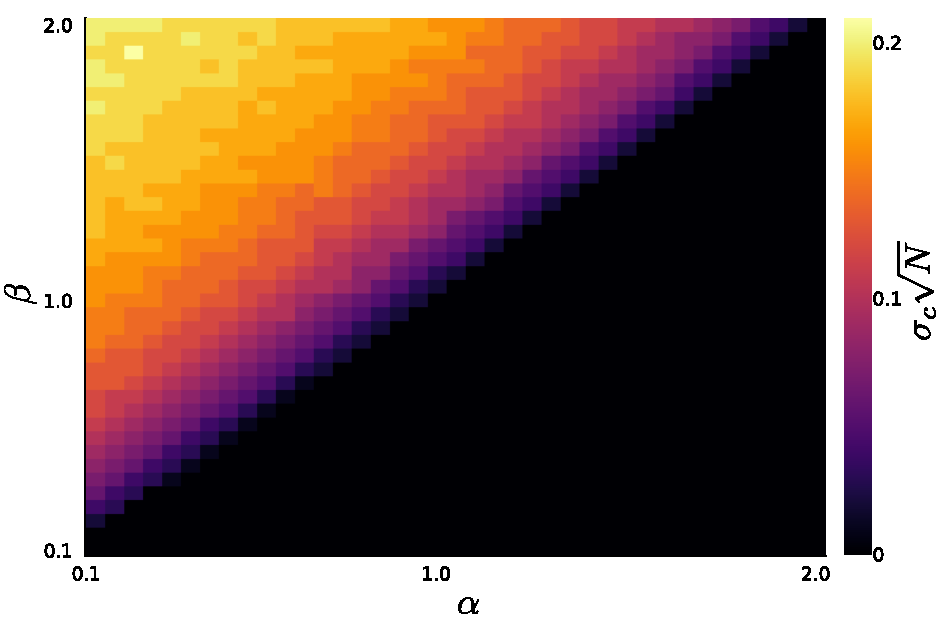
\includegraphics[width=.45\textwidth]{figs/alpha-beta.pdf}
    \caption{The ``May" and ``anti-May" phases described in the
    case of uniform interactions are robust with respect to random interactions.
    Here we simulated system~\eqref{dynamics} in the power law case for a fixed value of
    $\mu=\mu_s=10^{-2}$, $\gamma=1$, $N=100$ and $100$ replicates 
    and evaluated $\sigma_c$, defined here as
    the value above which full stable coexistence is less probable than 50\%,
    at varying $\alpha$ and $\beta$.
    No amount of heterogeneity is allowed in the lower triangle because we have $\mu=\mu_s$, while an increasing value of $\sigma_c$
    is found as $\beta$ becomes bigger than $\alpha$.
    We stress that the existence of a finite $\sigma_c\sqrt{N}$ above which instability is triggered also in the upper triangle,
    does not imply that increasing $N$ will destabilize the system, because $\mu N$ would also change.
    }
    \label{fig: alpha-beta}
\end{figure}
At equilibrium, we can write
\begin{equation}
    x_*^{\alpha-\beta} - A_s x_*^{\gamma}= \big( \mu N \langle x_*^{\gamma}\rangle + \sigma \sqrt{N\langle x_*^{2\gamma}\rangle}\xi\big) \, ,
\end{equation} 
where $\xi$ is now a standard normal random variable.
The equation above can be solved for $x_*$ for specific values of
$(\alpha-\beta)/\gamma$, or if $A_s=0$.
(In the following we show that neglecting $A_s$ even when it is not zero does not affect noticeably the quality of the approximation.) In this case the stationary solution is given by 
\begin{equation} \label{eq: cavity solution}
    x_* = \left( \mu N \langle x_*^{\gamma}\rangle + \sigma \sqrt{N\langle x_*^{2\gamma}\rangle}\xi\right)^{1/(\alpha-\beta)} \, .
\end{equation}
The equilibrium distribution $P(x_*)$ can then be obtained as the pushforward of the distribution of $\xi$: 
\begin{equation}\label{eq: dist general}
    P(x_*)=\frac{|\alpha-\beta|x_*^{\alpha-\beta-1}}{\sqrt{2\pi\sigma^2 N\langle x_*^{2\gamma}\rangle}}
    \exp{\left\{-\frac{(x_*^{\alpha-\beta}-\mu N\langle x_*^{\gamma}\rangle)^2}{2\sigma^2N\langle x_*^{2\gamma}\rangle}\right\}} \, ,
\end{equation}
where the expectation values must be computed self-consistently. 

Equipped with the equilibrium distribution $P(x^*)$, we can compute, for given $N$ and $\mu$, the maximal heterogeneity $\sigma_c$ consistent with the linear stability condition $N\langle (\sigma/\psi(x^*))^2\rangle < 1$ holds. 

Let us focus on the choice $\alpha=1$, $\beta=3/2$ and $\gamma=1$, with $A_s=0$.  
In this case the first and second moments formally diverge.
This is not truly problematic because we are dealing with large, but \emph{finite} populations.
Following~\cite{Cui2020,Hatton2023} and assuming $\sigma \sqrt{N\langle x_*^2\rangle}\ll \mu N \langle x_* \rangle$, we can expand the solution~\eqref{eq: cavity solution} to first order in $\sigma \sqrt{N\langle x_*^2\rangle}$, and approximate~\eqref{eq: dist general} with a Gaussian distribution with moments $\langle x_*\rangle=(\mu N)^{-2/3}$ and $\langle x_*^2\rangle=(\mu N)^{-4/3}/(1-4(\mu N)^{-2}\sigma^2N)$. 

The result is plotted against simulations in Fig.~\ref{fig: cavity sol.}. We show both the exact solution~\eqref{eq: dist general} (where integration for the moments has been performed up to a maximum value above which no equilibrium value should be found) and the Gaussian approximation. Simulations correspond to $A_s=\mu$, showing that neglecting the $A_s$ term in analytical expressions does not introduce a significant error. 


The properties of large random dynamical systems is often portrayed in often portrayed in the $(\sigma \sqrt{N},\mu N)$ plane \cite{bunin2017ecological}. Everything else fixed, an increase of the number of degrees of freedom $N$ moves the system along a square-root trajectory in that plane. In the GLV model, the boundary between the stable and unstable parameter regions is the horizontal line $\sigma_c\sqrt{N} = \mu_s$ \cite{bunin2017ecological}, hence stability is never possible at large $N$. 

In Fig.~\ref{fig: stability line + sims} we plot the stability condition $N\langle (\sigma/\psi(x^*))^2\rangle < 1$ for $\alpha = 1$, $\beta = 3/2$ derived from \eqref{eq: dist general} (solid line) together with results from simulations (shading). Here, because the boundary between the stable and unstable phases is a straight line with positive slope, increasing $N$ will eventually bring the system in the stable region. This behavior corresponds to the ``anti-May" phase defined previously. 








Finally, Fig.~\ref{fig: alpha-beta} shows results of simulations for $\sigma_c\sqrt{N}$ in the $(\alpha,\beta)$ plane, at fixed $\mu N$ and $\gamma = 1$. (Numerically, we define $\sigma_c\sqrt{N}$ as the value of $\sigma$ above which full stable coexistence has a probability lower than $50\%$.) In these simulations we use $\mu_s = \mu$, which would never be stable in the GLV model. Fig.~\ref{fig: alpha-beta} illustrates the transition between a ``May" phase for $\alpha \geq \beta$ and an ``anti-May" phase for $\alpha < \beta$, showing that our analytical results are robust to heterogeneous interactions.

%Conclusion
\paragraph*{}
\emph{Discussion.---}The relationship between complexity and stability in high-dimensional dynamical systems has been a longstanding puzzle, in ecology and in other fields. 
In this letter, we have showed that the condition $\sigma\sqrt{N}< \mu_s - \mu$ (popularized by May's slogan ``complexity begets instability") does not provide a complete picture of the relationship between complexity and stability. 
In particular, we have seen that generalized Lotka-Volterra model, often cited in support of May's prediction, corresponds to a special cancellation in the more general stability condition $N\langle (\sigma/\psi)^2\rangle < 1$.
In models where self-interactions grow faster than cross-interactions, the opposite behavior is observed: stability becomes \emph{more} likely with increasing diversity $N$.

Future work can look at the case where two-body interactions are not separable, or include higher order interaction to generalize the results in Ref. \cite{Gibbs2022} based on the GLV model. 

\medskip

\begin{acknowledgments}
We thank Ian Hatton, Matthieu Barbier and Ada Altieri for productive discussions on ecological power laws and the diversity-stability debate, and Vadim Karatayev and Daniel Reuman for feedback on the manuscript.
Funding for this work was provided by the Alexander von Humboldt Foundation in the framework of the Sofja Kovalevskaja Award endowed by the German Federal Ministry of Education and Research.
O.M. was partly supported by NSF BIO OCE grant 2023473.
\end{acknowledgments}

\medskip

\bibliography{beyond-may}
\bibliographystyle{unsrt}

\end{document}